%document
\documentclass[10pt]{beamer}
%theme
\usetheme{metropolis}
% packages
\usepackage{color}
\usepackage{listings}
\usepackage[main=ngerman, USenglish]{babel}
\usepackage[utf8]{inputenc}
\usepackage{multicol}
\usepackage{csquotes}


% color definitions
\definecolor{mygreen}{rgb}{0,0.6,0}
\definecolor{mygray}{rgb}{0.5,0.5,0.5}
\definecolor{mymauve}{rgb}{0.58,0,0.82}
\definecolor{paleorange}{HTML}{CC7832}

\lstset{
    backgroundcolor=\color{white},
    % choose the background color;
    % you must add \usepackage{color} or \usepackage{xcolor}
    basicstyle=\footnotesize\ttfamily,
    % the size of the fonts that are used for the code
    breakatwhitespace=false,
    % sets if automatic breaks should only happen at whitespace
    breaklines=true,                 % sets automatic line breaking
    captionpos=b,                    % sets the caption-position to bottom
    commentstyle=\color{mygreen},    % comment style
    % deletekeywords={...},
    % if you want to delete keywords from the given language
    extendedchars=true,
    % lets you use non-ASCII characters;
    % for 8-bits encodings only, does not work with UTF-8
    frame=single,                    % adds a frame around the code
    keepspaces=true,
    % keeps spaces in text,
    % useful for keeping indentation of code
    % (possibly needs columns=flexible)
    keywordstyle=\color{blue},       % keyword style
    % morekeywords={*,...},
    % if you want to add more keywords to the set
    numbers=left,
    % where to put the line-numbers; possible values are (none, left, right)
    numbersep=5pt,
    % how far the line-numbers are from the code
    numberstyle=\tiny\color{mygray},
    % the style that is used for the line-numbers
    rulecolor=\color{black},
    % if not set, the frame-color may be changed on line-breaks
    % within not-black text (e.g. comments (green here))
    stepnumber=1,
    % the step between two line-numbers.
    % If it's 1, each line will be numbered
    stringstyle=\color{mymauve},     % string literal style
    tabsize=4,                       % sets default tabsize to 4 spaces
    % show the filename of files included with \lstinputlisting;
    % also try caption instead of title
    language = Java,
	showspaces = false,
	showtabs = false,
	showstringspaces = false,
	escapechar = ,
        morecomment=[s][\textcolor{paleorange}]{@}{\ },
}

\def\ContinueLineNumber{\lstset{firstnumber=last}}
\def\StartLineAt#1{\lstset{firstnumber=#1}}
\let\numberLineAt\StartLineAt



\newcommand{\codeline}[1]{
        \alert{\texttt{#1}}
}

\setmonofont{Fira Code}

% This Document contains the information about this course.

% Authors of the slides
\author{Marcus Köhler}

% Name of the Course
\institute{Java-Kurs}

% Fancy Logo
\titlegraphic{\hfill
\includegraphics[height=1.25cm]{../templates/fsr_logo_cropped}}

\usepackage{csquotes}

\title{Java}
\subtitle{Weitere Programmierkonzepte in Java}
\date{\today}

\begin{document}

\begin{frame}
    \titlepage
\end{frame}

\begin{frame}{Überblick}
    \setbeamertemplate{section in toc}[sections numbered]
    \tableofcontents
\end{frame}

\section{Casting}
\subsection{Was ist Casting?}

\begin{frame}[fragile]{Was ist Casting?}
    Bei einigen Programmabläufen in Java ist es nötig, eine Referenz oder einen primitiven Datentypen in einen anderen Typ umzuwandeln.
    Hierzu gibt es in Java(wie auch in den meisten anden C-ähnlichen Sprachen) das sogenannte \textit{Casting} bzw. \textit{Typecasting}.
    Eine Variable bzw. Referenz wird gecastet, indem man den \enquote{Zieltyp} in Klammern vor das Statement setzt, das konvertiert werden soll:
    \begin{lstlisting}[gobble=8]
        int dividend = 42;
        int divisor = 8;

        float res = (float)dividend/divisor;
        System.out.println(res); //prints 5.0 because int-division is whole number division
    \end{lstlisting}
\end{frame}

\subsection{Warum casten?}
\begin{frame}[fragile]{Warum casten?}
    Gerade in der Verwendung von Polymorphie muss oft casting angewendet werden, wenn man mehr als die Methoden des Typs der Referenz verwenden will:
    \begin{lstlisting}[gobble=8,basicstyle=\ttfamily\scriptsize]
        Object objReference = new ArrayList<Integer>();
        //objReference can only access methods defined in Object
        objReference.add(9); //won't compile

        Collection<Integer> colReference = (Collection)objReference;
        //colReference can also access the methods defined in Collection
        colReference.listIterator(); //won't compile

        List<Integer> listReference = (List)objReference;
        //listReference can access all methods that are defined in List
        listReference.add(5, 9); //adds 9 at index 5; works just fine
    \end{lstlisting}
\end{frame}

\begin{frame}[fragile]{Warum casten?}
    Es ist auch möglich, nur einzelne Teile eines Statements zu casten, indem man den \enquote{zu castenden} Teil(inkl. des Castings an sich) mit Klammern zusammenfasst:
    \begin{lstlisting}[gobble=8]
        int dividend = 42;
        float divisor = 8;

        float res = ((float)dividend)/divisor; // float/float division because of casting
        System.out.println(res) // prints 5.25, the correct result
    \end{lstlisting}
\end{frame}


\subsection{Guidelines}

\begin{frame}{Guidelines für Casting}
    Beim Casting sollte man einige grundlegende Regeln beachten:
    \begin{itemize}[<+->]
        \item Bei primitiven Datentypen funktioniert Casting nur, wenn dabei keine Informationen verloren gehen:\\
            \texttt{int -> float} ist erlaubt, \texttt{float -> int} nicht
        \item Bei Objekten muss das \enquote{Quellobjekt}: \\
            \begin{itemize}
                \item eine Instanz des Zieltyps oder einer seiner Subklassen sein, falls der Zieltyp eine Klasse ist
                \item eine Instanz einer Klasse K(oder einer Subklasse von K) sein, wobei K das Interface implementiert, falls der Zieltyp ein Interface ist
            \end{itemize}
    \end{itemize}
\end{frame}

\section{Rekursion}
\subsection{Was ist Rekursion?}

\begin{frame}{Was ist Rekursion?}
    \begin{columns}[T]
        \begin{column}{.5\textwidth}
            \onslide<+->{\textit{Rekursion} bezeichnet eine Funktion bzw. eine Lösungsstrategie,
            die sich selbst wieder aufruft, meistens mit einem Subset der ursprünglichen Daten.\\
            \medskip
            Dies passiert so oft, bis entweder ein sogenannter \textit{Basecase} auftritt,
            für den eine Lösung bekannt ist, oder aber keine Lösung gefunden werden kann
            (oder eine \texttt{StackOverflowException} auftritt).}
        \end{column}
        \begin{column}{.5\textwidth}
            \onslide<+->{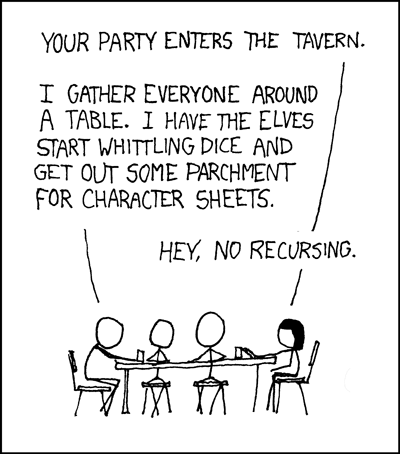
\includegraphics[width=\textwidth]{/home/marcus/git/progcourse/java/images/tabletop_roleplaying.png}
            \tiny{\url{https://xkcd.com/244}}}
        \end{column}
    \end{columns}
\end{frame}

\subsection{Beispiel}

\begin{frame}[fragile]{Rekursion:Beispiel}
    Ein klassisches Beispiel für Rekursion ist eine Funktion, die die n-te Zahl der Fibonacci-Folge berechnet:
    \begin{lstlisting}[gobble=8]
        public int fibonacci(int n) {
            if(n < 0) throw new IllegalArgumentException();
            if(n == 0 || n == 1) return 1; //define basecase
            return fibonacci(n-1) + fibonacci(n-2); //recursive call
        }
    \end{lstlisting}
    \vfill
    \onslide<2->{\centerline{\texttt{->DEMO<-}}}
\end{frame}

\section{Lambdas(Java 8+)}
\subsection{Lambdas‽}

\begin{frame}[fragile]{Lambdas?}
    \textit{Lambdas} sind Javas Implementierung von sogenannten \textit{anonymen Funktionen}. \\
    Im Klartext bedeutet das, dass man mittels Lambdas Funktionen als Parameter an Methoden übergeben kann. \\
    \pause
    Ein Lambda hat die Form \texttt{<Argument> -> <Funktion>}:
    \begin{lstlisting}[gobble=8]
        List<Integer> intList = new ArrayList<>();
        intList.add(1);
        intList.add(3);

        Iterator<Integer> iter = intList.iterator();

        iter.forEachRemaining(i -> System.out.print(i + " ")); 
        //prints 1 3
    \end{lstlisting}
\end{frame}

\begin{frame}[fragile]{Lambdas?}
    In einigen Fällen ist es notwendig, mehr als eine Funktion auf einmal auf dem Argument anzuwenden. Hierzu kann man auch mehrere Statements und das \texttt{return} Keyword verwenden. Dabei muss man die Funktion in {} packen:
    \begin{lstlisting}[gobble=8]
        //same setup as before
        iter.forEachRemaining(i -> {int sq = i*i;
                                    System.out.print((sq+10));}); 
        //prints 11 19
    \end{lstlisting}
    Dieser Code ist äquivalent zu folgendem:
    \begin{lstlisting}[gobble=8,basicstyle=\ttfamily\scriptsize]
        private void printSquarePlusTen(int i) {
            int sq = i*i;
            System.out.println((sq+10));
        }

        iter.forEachRemaining(this::printSquarePlusTen) 
        //:: is the Method reference Operator
        //this::printSquarePlusTen is equivalent to i -> printSquarePlusTen(i)
    \end{lstlisting}
\end{frame}

\subsection{Anwendungen von Lambdas}

\begin{frame}[fragile]{Lambdas!}
    Lambdas werden häufig in \texttt{Streams} eingesetzt. Streams sind eine neue Strategie(seit Java 8), über \texttt{Collections} zu iterieren:
    \begin{lstlisting}[gobble=8,basicstyle=\ttfamily\scriptsize]
        List<String> stringList = new Linkedlist<>();
        stringList.add(Arrays.asList("Peter", "Paul", "Petra")); //shorthand to add multiple elements at once
        Stream<String> stringStream = stringList.stream(); //"streams" the contents of the list
        
        stringStream = stringStream.filter(s -> s.length() == 5); 
        stringStream = stringStream.map(s -> s.replace('e', '@'));
        stringStream.forEach(System.out::println); //prints P@t@r P@tra
    \end{lstlisting}
    \pause
    Durch Verkettung von Methodenaufrufen kann man diesen Code auf den folgenden reduzieren:
    \begin{lstlisting}[gobble=8,basicstyle=\ttfamily\scriptsize]
        List<String> stringList = new Linkedlist<>();
        stringList.add(Arrays.asList("Peter", "Paul", "Petra"));
        
        stringList.stream().filter(s -> s.length() == 5)
                            .map(s -> s.replace('e', '@'))
                            .forEach(System.out::println); 
    \end{lstlisting}
    \onslide<3->{\centerline{\texttt{->DEMO<-}}} 
\end{frame}

\section{Übung}

\begin{frame}{Übung}
    \center
    \large{
        1. (Rekursion) Implementiere eine Funktion, die die Quersumme einer Zahl berechnet, mittels Rekursion. \\
        \medskip
        2. (Lambdas/Streams) Implementiere eine Funktion, die die Inhalte einer Liste ausgibt \\
        a) mittels Iterators und \texttt{while} \\
        b) mithilfe von Streams und Lambdas.
    }
\end{frame}

\end{document}
